\documentclass[oneside,a4paper,12pt]{book}

\usepackage[margin=1in]{geometry}
\usepackage{titlesec}
\usepackage{lipsum} 
\usepackage{xcolor} 

\usepackage{tikz}
\usepackage{subcaption}
\usepackage{ifthen}
\usepackage{tabularx}

\usepackage{fancyhdr}
\usepackage{lastpage}

\usepackage{fixltx2e}

\usepackage{amsmath}
\usepackage{amssymb}
\usepackage{booktabs}

\usepackage{amsthm}
\usepackage{ulem}
\usepackage{todonotes}

\usepackage{algpseudocode}
\usepackage{algorithm2e}

\definecolor{R}{RGB}{220,20,60}
\definecolor{B}{RGB}{39,64,239}
\definecolor{G}{RGB}{0,139,69}
\definecolor{orange}{rgb}{1,0.5,0}

\newcommand{\red}[1]{{\textcolor{R}{#1}}}
\newcommand{\blue}[1]{{\textcolor{B}{#1}}}
\newcommand{\green}[1]{{\textcolor{G}{#1}}}

\usepackage[hidelinks]{hyperref}
\hypersetup{linktocpage}

\begin{document}

\pagestyle{fancy}
\lhead{\footnotesize \parbox{11cm}{Cryptography A Notes} }
\lfoot{\footnotesize \parbox{11cm}{Shared}}
\cfoot{}
\rhead{\footnotesize Lecture Notes}
\rfoot{\footnotesize Page \thepage\ of \pageref{LastPage}}
\renewcommand{\headheight}{24pt}
\renewcommand{\footrulewidth}{0.4pt}

\titleformat{\chapter}[display]
  {\normalfont\normalsize\bfseries\LARGE}
  {\chaptertitlename~\thechapter}{1pc}
  {{\color{brown}\titlerule[2pt]}\vspace{1pc}\MakeUppercase}
    \titleformat{name=\chapter,numberless}[display]
  {\normalfont\normalsize\bfseries\LARGE}{}{1pc}
  {\MakeUppercase}
  
  
  
\newcounter{cryptogamearrows}
\newenvironment{cryptogame}[1]{
    \setcounter{cryptogamearrows}{0}
    \begin{center}
        \begin{tikzpicture}
            \node at (-1,0.75) {#1};
}{
            \draw [thick] (0.6,0.1) rectangle (1.9,0.35-0.5*\arabic{cryptogamearrows});
            \node at (1.25,0.2-0.25*\arabic{cryptogamearrows}) {\textbf{A}};
        \end{tikzpicture}
    \end{center}
}
\newcommand{\cgamearrow}[2]{\node [left] at (0,0-0.5*\arabic{cryptogamearrows}) {#1};\draw [thick][#2] (0,0-0.5*\arabic{cryptogamearrows}) -- (0.5,0-0.5*\arabic{cryptogamearrows});\stepcounter{cryptogamearrows}}
\newcommand{\cgameright}[1]{\cgamearrow{#1}{->}}
\newcommand{\cgameleft}[1]{\cgamearrow{#1}{<-}}  

\newcommand{\cbox}[2]{\begin{tikzpicture}\node [rectangle, draw, fill=#1, text centered, rounded corners] {#2};\end{tikzpicture}}
\newcommand{\gbox}[1]{\cbox{blue!20}{#1}}

\newcommand{\boldcbox}[2]{\begin{tikzpicture}\node [rectangle, draw, thick, fill=#1, text centered, rounded corners] {\textbf{#2}};\end{tikzpicture}}

\newboolean{indcca}\newboolean{indcpa}\newboolean{indpass}
\newboolean{owcca}\newboolean{owcpa}\newboolean{owpass}

\newcommand{\clearattackcolours}{
    \setboolean{indcca}{false}\setboolean{indcpa}{false}\setboolean{indpass}{false}
    \setboolean{owcca}{false}\setboolean{owcpa}{false}\setboolean{owpass}{false}
}

\newcommand{\comment}[1]{}
\newcommand{\attackpasscolour}{green}
\newcommand{\ttackfailcolour}{red!80}
\newcommand{\condbox}[3]{\ifthenelse{ \equal{#1}{#3}
                            }{
                                \ifthenelse{\boolean{#1}}{\boldcbox{\attackpasscolour}{#2}}{\bold{\ttackfailcolour}{#2}}
                            }{
                                \ifthenelse{\boolean{#1}}{\cbox{\attackpasscolour}{#2}}{\cbox{\ttackfailcolour}{#2}}
                            }
                        }

\newcommand{\attacktable}[1]{
    \clearattackcolours
    \setboolean{#1}{true}
    \ifthenelse{\boolean{indcca}}{\setboolean{indcpa}{true}}{}
    \ifthenelse{\boolean{indcpa}}{\setboolean{indpass}{true}}{}
    \ifthenelse{\boolean{indcca}}{\setboolean{owcca}{true}}{}
    \ifthenelse{\boolean{indcpa} \OR \boolean{owcca}}{\setboolean{owcpa}{true}}{}
    \ifthenelse{\boolean{indpass} \OR \boolean{owcpa}}{\setboolean{owpass}{true}}{}
    \begin{tabular}{ccccc}
        \condbox{indcca}{IND-CCA}{#1} & $\rightarrow$ & \condbox{indcpa}{IND-CPA}{#1} & $\rightarrow$ & \condbox{indpass}{IND-PASS}{#1}\\
        $\downarrow$ && $\downarrow$ && $\downarrow$ \\
        \condbox{owcca}{OW-CCA}{#1} & $\rightarrow$ & \condbox{owcpa}{OW-CPA}{#1} & $\rightarrow$ & \condbox{owpass}{OW-PASS}{#1}\\
    \end{tabular}
}

\newcommand{\attacktabletwo}[2]{
    \clearattackcolours
    \setboolean{#1}{true}
    \setboolean{#2}{true}
    \ifthenelse{\boolean{indcca}}{\setboolean{indcpa}{true}}{}
    \ifthenelse{\boolean{indcpa}}{\setboolean{indpass}{true}}{}
    \ifthenelse{\boolean{indcca}}{\setboolean{owcca}{true}}{}
    \ifthenelse{\boolean{indcpa} \OR \boolean{owcca}}{\setboolean{owcpa}{true}}{}
    \ifthenelse{\boolean{indpass} \OR \boolean{owcpa}}{\setboolean{owpass}{true}}{}
    \begin{tabular}{ccccc}
        \condbox{indcca}{IND-CCA}{#1} & $\rightarrow$ & \condbox{indcpa}{IND-CPA}{#1} & $\rightarrow$ & \condbox{indpass}{IND-PASS}{#1}\\
        $\downarrow$ && $\downarrow$ && $\downarrow$ \\
        \condbox{owcca}{OW-CCA}{#1} & $\rightarrow$ & \condbox{owcpa}{OW-CPA}{#1} & $\rightarrow$ & \condbox{owpass}{OW-PASS}{#1}\\
    \end{tabular}
}


\titleformat*{\paragraph}{\large\normalfont}

\title{Cryptography A - Lecture Notes}
\author{Shared}
\date{\today}
\maketitle
\tableofcontents
\mainmatter

\thispagestyle{fancy}
\renewcommand{\headheight}{24pt}
\renewcommand{\footrulewidth}{0.4pt}

\newcommand{\chaptersub}[2]{\chapter[#1]{#1 \\ \large{\textit{#2}}}}



\newcommand{\cm}{\red{m}}
\newcommand{\cc}{\blue{c}}
\newcommand{\cN}{\blue{N}}
\newcommand{\cp}{\red{p}}
\newcommand{\cq}{\red{q}}
\newcommand{\cd}{\red{d}}
\newcommand{\ce}{\blue{e}}
\newcommand{\ck}{\red{k}}
\newcommand{\cpk}{\blue{p}\blue{k}}
\newcommand{\csk}{\red{s}\red{k}}
\newcommand{\cK}{\red{k}}
\newcommand{\csig}{\blue{s}}

\newcommand{\csubm}[1]{\red{m}_\red{#1}}
\newcommand{\csubc}[1]{\red{c}_\red{#1}}
\newcommand{\csubcast}[1]{\red{c}_\red{#1}^\red{*}}
\newcommand{\ccast}{\red{c}^\red{*}}
\newcommand{\cmast}{\red{m}^\red{*}}
\newcommand{\csubk}[1]{\red{k}_\red{#1}}

\chapter{Introduction}
\section{Cryptography and Modern Cryptography}
    
    Classical cryptography was, until the 20th century, considered more of an art than a science as it had no real theory to rely upon.\\
    \\
    Modern cryptography, however, is much more formal and encompasses a great deal more than just secret communication. It also covers: message authentication, digital signatures, electronic auctions and elections, digital currency etc.\\
    \\
    It also differs by the places in which it is found; Classical cryptography was mainly used by the military and intelligence organisations, whilst modern cryptography is used in almost every computer system. It is used when accessing a secure website, when authenticating on a multi-user operating system etc.\\
    \\
    Definition: \textbf{Modern Cryptography is the scientific study of techniques for securing digital information, transactions, and distributed computations.}
    
\section{Principles of Secure Communication}
    There are two types of encryption systems: symmetric (\textbf{private key}, or classical) and asymmetric (\textbf{public key}) encryption. Both rely on these principles for secure communication.\\
    \\
    \textbf{Confidentiality}: An adversary cannot see which messages are transmitted, though they may see that something is being sent.\\
    \\
    \textbf{Authenticity}: An adversary cannot cause non-original messages to be accepted. This is related to but different from...\\
    \\
    \textbf{Integrity}: An adversary cannot alter messages in transit without the alteration being detected.\\

\section{Private Key Encryption}

    Private-key encryption implies both the sender and the receiver use the same secret key to encrypt and respectively decrypt the message.\\
    \\
    This method was useful for the military in the past as the two parties would be able to physically meet and decide upon a key whereas today achieving that is more difficult as the parties meeting would be inconvenient or impossible most times(think about online money transfers or user authentication).\\
    \\
    However, this method is still being applied in some scenarios like disk/file encryption where the same user at different points in time uses the same secret key to both read and write to a file. Private-key encryption is also widely used in conjunction with asymmetric methods.\\
    \\
    The private key encryption scheme is comprised of three algorithms:
    
    \begin{itemize}
      \item The key generation algorithm(\textit{Gen}) which is a probabilistic algorithm that outputs a key, $\ck$, chosen according to some distribution that is determined by the scheme.
      \item The encryption algorithm(\textit{Enc}) which takes as input a key $\ck$ and a plaintext message \textit{M} and outputs a cipher text \textit{C}: $Enc_\ck(M) = \cc;$
      \item The decryption algorithm(\textit{Dec}) which takes as input a key $\ck$ and a cipher \textit{C} and outputs the original message \textit{M}: $Dec_\ck(C) = \cm;$
    \end{itemize}
    
    Decrypting a cipher text using the appropriate key yields the original message or: $Dec_\ck(Enc_\ck(\cm))=\cm$.
    \\
    
% Not sure if this is the best place for this, but it is an important principle, so perhaps...
\section{Kerckhoff's Principle}
    Kerckhoff's principle is fundamental to cryptography. It is this: \textbf{``Security should rely solely on the secrecy of the key.''}.\\
    \\
    Arguments:
    \begin{itemize}
      \item It is much easier to maintain secrecy of a short key than a complex algorithm.
      \item Changing a disclosed key is much easier than changing a disclosed algorithm.
      \item In case more parties need to communicate it is easier to produce multiple keys than multiple algorithms.
    \end{itemize}
    Example of attack scenarios:
    \begin{itemize}
      \item Cipher-only attack
      \item Known-plaintext attack
      \item Chosen-plaintext attack
      \item Chosen-cipher attack
    \end{itemize}




\chapter{Classical Cryptography}

\section{Historical Ciphers and Their Cryptanalysis}

\begin{itemize}
    \item \textbf{Caesar cipher}\\\\
The encryption is done by rotating the letters of the alphabet by 3(A becomes D). The biggest problem
with this cipher is that the method is fixed and there is no key to speak of. Therefore anyone
learning the decryption algorithm would be able to get the initial message effortlessly.
    \item \textbf{The shift cipher}\\\\
This cipher is similar to the Caesar cipher but it introduces a secret key \textit{k} that is a number
between 0 and 25. The encryption is then done by shifting the letters by \textit{k} places.\\\\
\begin{math}Enc(m_{i}) = [(mi+k) mod 26];\\
Dec(c_{i}) = [(c_{i}-k) mod 26]\end{math};\\\\
This cipher is not secure as it can be easily broken by doing an exhaustive search. There are
only 26 possible keys therefore the cipher does not follow the insufficient key space principle
which says that any secure encryption scheme must have a key space that is not vulnerable to
exhaustive search. The number of possible keys must be very large (at least 2\textsuperscript{60} or 2\textsuperscript{70}).
    \item \textbf{Mono-alphabetic substitution}\\\\
The idea behind the mono-alphabetic substitution is to map each plaintext character to a
different cipher text character in an arbitrary manner. The keys space thus consists of all
permutations of the letters of the alphabet which is approximately 2\textsuperscript{88}, too big for an exhaustive search.\\
However this does not make it secure. Considering that the plain text message is written
in plain English we can calculate the frequency of each letter and then compare the cipher`s table of frequencies with the table of frequencies for the English language.
    \item \textbf{Improved attack on the shift cipher}\\\\
The initial approach was to try all possible keys and check which one gives a message that
``makes sense``. But sometimes it is hard to define what ``makes sense`` actually means. If the
initial message is not written in plain English it is hard to know which solution is the correct one.
There are cases though when the plain text message is not written in valid English but has the
letter distribution of such a text.\\
In this case we compute the following sum: \begin{math}I_j = \sum_{i=0}^{25} p^2*\approx0.065\end{math} where \textit{p\textsubscript{i}} is each letter`s frequency in the plain text with \begin{math}0<=i<=25\end{math}. We know that the letters are shifted by \textit{k} spaces, therefore \textit{q\textsubscript{i+k} = p\textsubscript{i}}. Now all we need to do is compute the sum \begin{math}I_j = \sum_{i=0}^{25} p_i*q_{i+j}\end{math} where \textit{q\textsubscript{i}} is each letter`s frequency in the cipher text and compare it to 0.0065. The \textit{j} for which I\textsubscript{j} is closest to 0.065 is the key. 

    \item \textbf{The Vigenere cipher}\\\\
The statistical attack on the mono-alphabetic substitution cipher was possible because the
mapping of each letter was fixed.\\
Consider the possibility when a letter is mapped to multiple letters. In this case the table of
frequencies would be irrelevant as the frequencies are very similar.
The Viginere cipher takes a repeated small string and forms the key which is then added to the
original message.\\
In order to simplify the breaking process we first need to identify the length of the key. If the
original message is written in plain English then we should look for repeated sequences of length
2 and 3 in the key. These will indicate us the appearances of common words like \textit{``the``} which
are in the same relative position of the small substring that is repeated, therefore the distance
between 2 such appearances would be a multiple of the length of the substring. Knowing this
we can assume that the greatest common divisor between the distances of such appearances is
either the length of the key or a multiple of it.\\
Knowing the key`s length the task is much simplified. We notice that we can split the initial text
in a number of substrings equal to the keys length(\textit{n}). This way the characters on positions \textit{1,n, 2n} etc. will be encrypted using the first character of the key, the positions \textit{2, n+1, 2n+1} etc. using the second character of the key and so on.\\
We now have \textit{n} different ciphers that are encrypted using the shift cipher with key \textit{K[i]}.
Therefore we need to decipher each string individually. Considering that we selected dispersed
characters from a plain English text, all the substrings will not be in plain English. Knowing this
we can now apply the method described above under \textit{``Improved attack on the shift cipher``}.
\end{itemize}


\section{Perfectly Secret Encryption}
\textbf{Definition:} An encryption scheme $(Gen,Enc,Dec)$ over a message space $M$ is perfectly secret if for every probability distribution over $M$, every message $m \in M$, and every ciphertext $c \in C$ for which $P(C=c)>0:$

$$P(M=m|C=c)=P(M=m)$$

In other words a scheme is perfectly secret if the distributions over messages and ciphertexts are independent.

\section{One Time Pad}
The one time pad is a good system to review because it is \textbf{totally secure} / perfectly secret, if used correctly. Sadly, it is difficult to use in the real-world.\\
\\
It works by XOR-ing the entire message by the cipher. This means that the cipher must be as long as the message, which is clearly a limitation in the real world --- encrypting your hard drive would require another hard drive of data for the cipher.\footnote{The XOR operations outputs a 0 bit at every position in which both operands have the same bit, and a 1 in positions where they differ.}\\
\\
The other limitation is the fact it can only be used once. This is because an adversary  can ask you to encrypt a message ($c=m\oplus k$). They can then use that to calculate the key, $k$,  because they have both $c$ and $m$ ($k=m\oplus c$). In practice, this means that if you know part of a message being sent, you can use that to calculate the bits of cipher in those positions.

\section{Shannon's Theorem}
...

\chapter{Cryptographic Definitions}


\section{The Three Principles of Modern Cryptology}

\begin{enumerate}
    \item Formulate a rigorous and \textbf{precise definition of security}.
    \item When a cryptographic system relies on an \textbf{unproven assumption}, it must be \textbf{precisely stated}. Furthermore, this assumption \textbf{must be minimal}.
    \item Cryptographic constructions must be accompanied by a \textbf{rigorous proof of security} with respect to the definition formulated in principle 1, revolving around the assumptions stated in principle 2.
\end{enumerate}

\subsection{Principle 1: Formulation of Exact Definitions}

\begin{itemize}
    \item \textbf{Why is this important?}
    \begin{itemize}
        \item \textbf{Importance for design:} We need to have a good understanding of our goal so that
we know when we achieve it. Sometimes our cryptographic system doesn't need to
be as efficient as possible, a simpler version being sufficient.
        \item \textbf{Importance for usage:} When we want to choose an existing cryptographic scheme
we need to have some sort of comparison criteria to be able to tell if it suffices our
application.
        \item \textbf{Importance for study:} For researching different types of cryptographic systems
we need to be able to compare them and measure their security level. Without
a rigorous proof of security the only performance attribute we can measure is
efficiency(which is not very accurate).
    \end{itemize}
    \item \textbf{How do we define security?}
    \begin{itemize}
        \item An encryption scheme is secure if no adversary can compute any function of the
plaintext from the cipher text.
        \item An encryption scheme is considered broken if an adversary learns some function of
the plaintext from the cipher text.
        \item The power of the adversary relates to assumptions regarding the actions the
adversary is assumed to be able to take, as well as the adversary`s computational
power.
    \end{itemize}
\end{itemize}

\subsection{Principle 2: Reliance on Precise Assumptions}

Most cryptographic constructions cannot be proven secure unconditionally, therefore it relies on some assumptions which must be precisely stated for the following reasons:

\begin{enumerate}
\item \textbf{Validation of the assumption} If the assumption being relied upon is not precisely stated and presented it cannot ber studied and potentially refuted.
\item \textbf{Comparison of schemes} If the assumptions used by two schemes are incomparable, then the one based on the better-studied or the simpler assumptions is preferred.
\item \textbf{Facilitation of proofs of security} A mathematical proof that ``the construction is secure if assumption is true'' cannot be provided without a precises statement of what the assumption is.
\end{enumerate}

\subsection{Principle 3: Rigorous Proofs of Security}

The first two principles lead naturally to this one. Most proofs in modern cryptography use the \textbf{reductionist} approach, that is, \textit{``Given the Assumption A is true, Construction C is secure according to the given definition.''}

\section{Cryptographic Games}

We can capture a notion of security by a picture representing a game played with adversary $A$. The games have one of two goals and the adversary has a range of powers.

\subsection{Indistinguishability (IND-Security)}

Indistinguishability is measure of security where by an adversary can give you two messages, and if you were to encrypt only one of them, he/she would not be able to know \textbf{which one you have encrypted}.\\
\\
Figure~\ref{fig:ind-sec-sym} shows the cryptographic game which captures this for a symmetric cryptographic scheme. $\csubm{0}$ and $\csubm{1}$ are the two messages the adversary gives you and the $\ccast$ is the ciphertext you computed of one of the messages. $b'$ is the answer the adversary gives. Note that $|\csubm{0}|=|\csubm{1}|$, since a difference in size would give the game away.\\
\begin{figure}[htp!]
    \centering
    \begin{subfigure}[b]{0.4\textwidth}
        \centering
        \begin{cryptogame}{$b\in \{0,1\}$}
            \cgameleft{$\csubm{m},\csubm{m}$}
            \cgameright{$\ccast=\textrm{Enc}_\ck(\csubm{b})$}
            \cgameleft{$b'$}
        \end{cryptogame}
        \caption{Symmetric Key  Case}
        \label{fig:ind-sec-sym}
    \end{subfigure}
    ~
    \begin{subfigure}[b]{0.4\textwidth}
        \centering
        \begin{cryptogame}{$b\in \{0,1\}$}
            \cgameright{$\cpk$}
            \cgameleft{$\csubm{0},\csubm{1}$}
            \cgameright{$\ccast=\textrm{Enc}_\ck(\csubm{b})$}
            \cgameleft{$b'$}
        \end{cryptogame}
        \caption{Public Key Case}
        \label{fig:ind-sec-pub}
    \end{subfigure}
    \caption{IND-Security Games}
    \label{fig:ind-sec}
\end{figure}
\\
Figure~\ref{fig:ind-sec-pub} gives the same but for public key encryption. $pk$ is the publicly available key, which all adversaries would have access to while trying to crack your message.\\
\\
A cryptographic system fails a game if an adversary can win the game more than chance.

\subsection{One-wayness (OW-Security)}

One-wayness is the property that an attacker, with only the ciphertext, \textbf{cannot decrypt the message}. The layout of the games used for this are in Figure~\ref{fig:ow-sec}.

\begin{figure}[htp!]
    \centering
    \begin{subfigure}[b]{0.4\textwidth}
        \centering
        \begin{cryptogame}{$\cm\in \mathbb{P}$}
            \cgameright{$\ccast=\textrm{Enc}_\ck(\csubm{b})$}
            \cgameleft{$m'$}
        \end{cryptogame}
        \caption{Symmetric Key  Case}
        \label{fig:ow-sec-sym}
    \end{subfigure}
    ~
    \begin{subfigure}[b]{0.4\textwidth}
        \centering
        \begin{cryptogame}{$b\in \{0,1\}$}
            \cgameright{$\cpk$}
            \cgameleft{$\csubm{0},\csubm{1}$}
            \cgameright{$\ccast=\textrm{Enc}_\ck(\csubm{b})$}
            \cgameleft{$b'$}
        \end{cryptogame}
        \caption{Public Key Case}
        \label{fig:ow-sec-pub}
    \end{subfigure}
    \caption{OW-Security Games}
    \label{fig:ow-sec}
\end{figure}

\subsection{Adversarial Powers}
These attacks also have defined `adversarial powers', where the adversary has access to specific oracles.
\begin{itemize}
    \item \textbf{Passive Attack}: Has no oracles --- all games above are passive attacks.
    \item \textbf{Chosen Plaintext Attack (CPA)}: The adversary can encrypt any mesage of his/her choosing.
    \item \textbf{Chosen Ciphertext Attack (CCA)}: The adversary can decrypt any message of his choosing, except he is not allowed to decrypt $\ccast$.
\end{itemize}
We assume that if an adversary has access to a decryption oracle, then they have access to the encryption one. This is apparently not true for one case we will see later... There is also no notion of a passive attack for public key encryption because the public key (which is used to encrypt) is public, so will always be accessible.

\section{Reductions}
We can make comparisons of problems by reducing one to another, there by defining one as `no harder' than the other. A reduction is where we can, in polynomial time, convert a problems into another one. We say \textbf{Problem A is no harder than Problem B} if we can convert Problem A into Problem B. This is written as \boldmath $A \leq_P B$ \unboldmath\\
\begin{figure}[htp!]
    \begin{center}
        \begin{tabular}{ccccc}
            \gbox{IND-CCA} & $\rightarrow$ & \gbox{IND-CPA} & $\rightarrow$ & \gbox{IND-PASS}\\
            $\downarrow$ && $\downarrow$ && $\downarrow$ \\
            \gbox{OW-CCA} & $\rightarrow$ & \gbox{OW-CPA} & $\rightarrow$ & \gbox{OW-PASS}\\
        \end{tabular}
    \end{center}
    \caption{Relationships between attacks}
    \label{fig:relations}
\end{figure}
\\
Some attacks are more powerful than others. Figure~\ref{fig:relations} show these relationships between the attacks. An arrow ($A \rightarrow B$) means $A$ is more powerful than $B$ and thus a proof that a system meets $A$'s notion of security, also proves it meets $B$'s.\\
\\
\textbf{IND-CCA is the de-facto} security definition we should accept. This means that the encryption must be probabilistic (i.e. encryption is a one-to-many function) because it could ask the oracle to encrypt $m_0$ and from that could win the game.


\section{Stream Ciphers}
The idea behind a stream cipher is to replace the (possibly) huge cipher needed for the Vernam scheme by a pseudo-random sequence which is `seeded` by a key of a more practical size. There's some confusion over whether the term `stream cipher' refers to the algorithm generating the stream or the entire encryption scheme. The term can use both, but the book accompanying the unit recommends you only use it for the algorithm
\begin{figure}
    %\includegraphic[width=\textwidth]{img/streamchipher.png}
    \caption{A stream cipher using a DFA where keys determine state update ($\csubk{1}$), initial state ($\csubk{2}$) and output filter ($\csubk{3}$)}
\end{figure}
\\
One model of a stream cipher is of a finite state machine, where the key provides the initial state, variables used to convert a keystream, $\csubk{i}$, to the next keystream, $\csubk{i+1}$. The ouput of the FSA is also XORed with a value taken from the key.\\
\\
One source for confusion may come from that fact that the slides use $\csubk{x}$ to for both the key values which are inputted into the stream cipher and for the keystream, which is the output of the stream cipher.\\
\\
Decryption is easy as both sender and receiver use key to generate the keystream of necessary size. This possible because the algorithm is deterministic, which, as meantioned later, is a source of weakness.



\chapter{Mathematics}
% Alternative title: kill me now. 
% I will buy the person that writes this section a Freddo. - Matt Bessey.
% Matt, you owe me a Freddo - Drum Ogilvie
    \section{Modular Arithmetic \& Groups}
    \subsection{Modular Arithmetic}
    Modular arithmetic is a bit odd at first, but you get used to it. It's all about remainders, really; we express modular relations in the following form:\\
    \begin{figure}
    \centering
        $$
        X \equiv \textit{Y \emph{\textbf{MOD}} Z}
        $$
    \end{figure}\\
    
    Where $X$ is any old number and $Z$ is the `Modulus'. Y is the remainder of the integer division of $X$ by $Z$, the result of an operation expressed in many languages (including C) as $X \% Z$. Simples.\\
    \\
    This leads us nicely onto groups.

    \subsection{Groups}
    A mathematical group is a combination of a set and an operation. So in our case, we use the set of remainders under some Modulus, defined thusly:
    \begin{figure}
    $$
        (\mathbb{Z}/N\mathbb{Z}) = \{0,..., N - 2, N - 1 \}
    $$

    \section{Multiplicative Inverse}
    The `inverse' for a group member is another member of the same group that when used as the second argument for the operation gives the result of the identity for that operation.\\
    \\
    In this case, the operation is multiplication, the multiplicative identity is 1, and our group is usually numbers Modulo N. So the inverse of one number Mod N is another number less than N, that when you multiply them together you get a number which is 1 Mod N. Still here? Still awake? Stay with me, soldier.
    
    \section{Greatest Common Divisor}
    Say you've got two numbers. What is the biggest factor that they both share? BOOM. 
    
    \section{Euler Phi Function}
    Also known as Euler's Totient Function
        
    \section{Lagrange's Theorem}
    
        \subsection{Fermat's Little Theorem}
        
    \section{Fields}
    
    \section{Chinese Remainder Theorem}
    
    \section{One Way Functions}
    
    %%%%%%%%%%%%%%%%%%%%%%%%%%%%%%%%%%%%%%%%
    % There's actually a few more sections %
    %%%%%%%%%%%%%%%%%%%%%%%%%%%%%%%%%%%%%%%%
%This chapter can go wherever, but here seemed appropriate

\chaptersub{Symmetric Modes}{Private Key Cryptography}

\section{Block Cipher Modes}\label{sec:blockciphermodes}
    A \textbf{block cipher} is type of encryption based on \textbf{permutation}, where they key, $\{0,1\}^k$, defines a transposition of bits in the block to the encrypted, $\{0,1\}^b$. The block is a proportion of the message.\\
    \\
    DES was the first civilian block cipher and was developed at IBM in the 1970s. When the US government adopted it, they recommended the following four ways to use it, these are now used with any block cipher.
    \begin{itemize}
        \item Electronic Code Book
        \item Cipher Block Chaining
        \item Counter
        \item ...
    \end{itemize}
    
    \subsection{Electronic Code Book}
    This is a very simple, it \textbf{divides} the message into blocks of size $b$, pads the last one, and \textbf{encrypts them all individually}. A block cipher using ECB is only OW-CPA, as Figure~\ref{fig:ecb-attacktable} says. This the terrible!\\
    \begin{figure}[htp!]
    \centering
    \attacktable{owcpa}
    \caption{Security Models ECB passes}
    \label{fig:ecb-attacktable}
    \end{figure}
    \\
    The weakness of this mode is in the fact that the blocks of encrypted independently. This is the basis for the two attacks below, but it also means it's susceptible to \textbf{block replay}. That is where an adversary edits a bit knowing how it will affect the decrypted message. If I knew you were sending me some money, and I knew the block containing the amount you were transferring, I could change that block in the hope I would end up with a larger transaction. This could be fixed with a checksum. ECB has one positive that an error in the cipher text will not propagate to other blocks when decrypted.\\
    \\
    \textbf{Proving a cryptographic system passes a security model is beyond this scope of this course}, but you should be able to give an intuitive reason. It passes OW-CPA because, with only an encryption oracle, you would have to brute-force every possible message to match it with the ciphertext. We can always make $b$ large enough so that this is not possible\footnote{This might be possible if you knew the context of the message, if you understand what is being sent and the domain of possible values of a block is relatively small. This is simply poor implementation of the encryption, however, and we don't worry about that.}. Note that all the proofs for block cipher modes assume we are using a `perfect block cipher'.\\
    \\
    \textbf{OW-CCA Example:} We can win an OW-CCA game by kind of cheating in the following way. If we have a decryption oracle, we can decrypt anything that is not the message. Since the blocks are independent, we can simply split the message in half and decrypt both individually and then concatenate the result.\\
    \\
    \textbf{IND-PASS Example:} In an Indistinguishability game we decide the message (of which one will be encrypted). Again we use the fact that the blocks are encrypted independently, and give one of the message as a bit string concatenated onto itself, $m_0=b_1||b_1$. The ciphertext can be split into two equal bit strings in the same way, then it was that message.
    
    
    
    \subsection{Cipher Block Chaining}
    Cipher Block Chaining removes a lot of the problems with the ECB by XORing each block with the previously encrypted block --- incorporating a dependence on the previous block. The first block of the ciphertext is called the \textbf{Initalisation Vector} (IV), and is what the first block of the message is XOR-ed with.\\
    \begin{figure}[htp!]
        \centering
        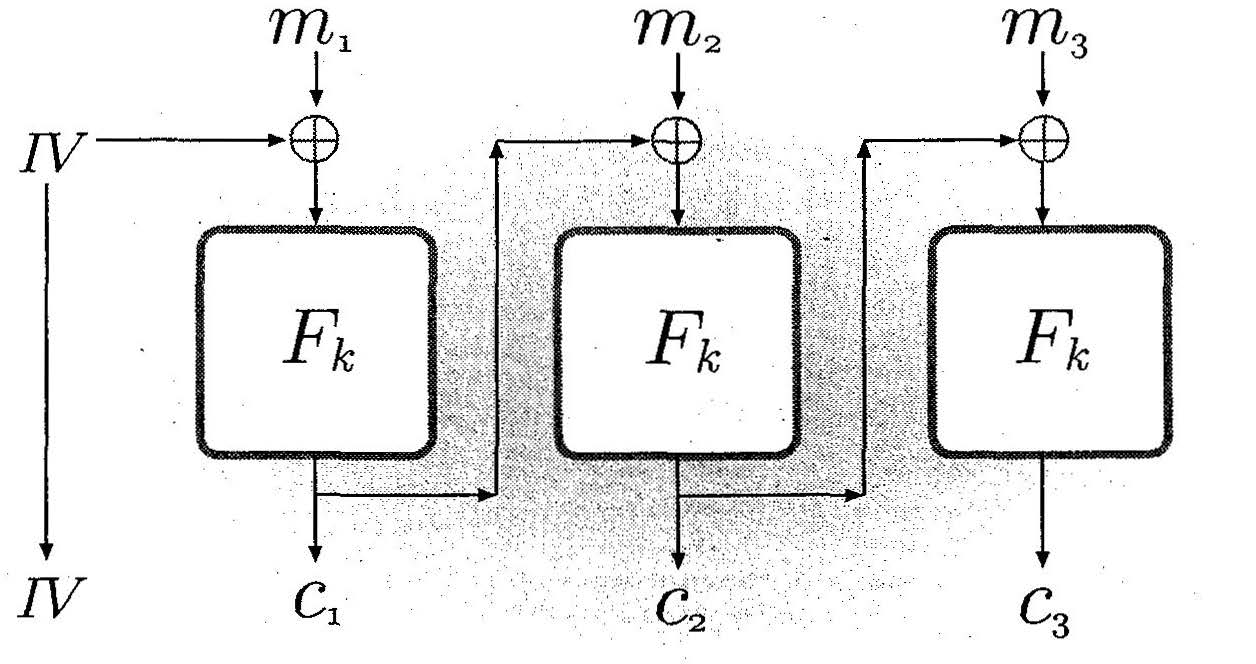
\includegraphics[width=10cm]{img/cbc}
        \caption{Diagram of CBC encrypting}
    \end{figure}
    \\
    More formally:\nopagebreak
    \begin{center}
    \begin{tabular}{lll}
    \textbf{Encryption}:                                        && \textbf{Decryption}\\
    $\csubc{0} = IV$                                                  && $IV = \csubc{0}$\\
    $\csubc{1} = Enc_\ck(\csubm{1} \oplus IV)$                                && $\csubm{1} = Dec_\ck(c_1) \oplus IV$\\
    $\csubc{i} = Enc_\ck(\csubm{i} \oplus \csubc{i-1}) \textrm{ for } i > 1$      && $\csubm{i} = Dec_\ck(c_i) \oplus \csubc{i-1} \textrm{ for } i > 1$\\
    \end{tabular}
    \end{center}
    \begin{figure}[htp!]
        \centering
        \attacktable{indcpa}
        \caption{Security of Models CBC}
        \label{fig:cbc-attacktable}
    \end{figure}
    Note that $IV$ is sent unencrypted, because it is needed for decryption. This can seem pointless, but if it is generated randomly every time, then it means that encryption is probabilistic. CBC is OW-CPA and IND-CPA but not OW-CCA or IND-CCA.\\
    \begin{figure}[htp!]
        \centering
        \begin{subfigure}[b]{0.3\textwidth}
            \centering
            
\includegraphics[width=\textwidth]{img/Tux.jpg}
            \caption{Original Image\\~}
        \end{subfigure}
        \begin{subfigure}[b]{0.3\textwidth}
            \centering
            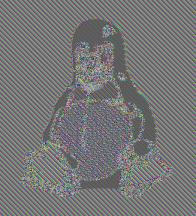
\includegraphics[width=\textwidth]{img/Tux_ecb.jpg}
            \caption{Encrypted using ECB\\~}
        \end{subfigure}
        \begin{subfigure}[b]{0.3\textwidth}
            \centering
            
\includegraphics[width=\textwidth]{img/Tux_secure.jpg}
            \caption{Encrypted using Chaining}
        \end{subfigure}
        \caption{Bitmap image of Tux being encrypted using ECB and using another method that uses chaining.}
        \label{fig:tux}
    \end{figure}
    \\
    \textbf{With a decryption oracle, CBC will fail} because of the same trick used before --- we can ask to oracle to decrypt the ciphertext with extra blocks on the end.
    
    
    
    \subsection{Counter Mode}
    Counter mode basically uses a stream cipher to generate a pseudo-random bit-string which can be one-time-padded with message. As Figure~\ref{fig:ctr} shows, generates a $IV$ ($IV \leftarrow \{0,1\}^n$) and increments this by one for every block. The $IV+n$ values are then put through the block cipher to generate the bit-string. In all the material, the $IV$ is refereed to as $ctr$ for this algorithm.\\
    \begin{figure}[htp!]
        \centering
        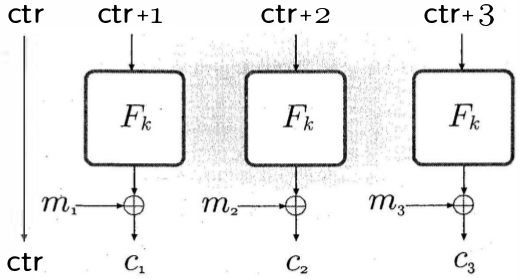
\includegraphics[width=0.5\textwidth]{img/ctr.png}
        \caption{Diagram of CTR mode}
        \label{fig:ctr}
    \end{figure}
    \\
    Formally:
    \begin{center}
        \begin{tabular}{lll}
            \textbf{Encryption:} && \textbf{Decryption:}\\
            $\csubc{0} = IV$ && $IV = \csubc{0}$\\
            $\csubc{i} = Enc_\ck(IV + i) \oplus \csubm{i}$ && $m_i = Enc_\ck(IV + i) \oplus \csubc{i}$
        \end{tabular}
    \end{center}
    CTR mode passes the same security modes as CBC (Figure~\ref{fig:ctr-attacktable}). But it has one positive over CBC: decrypting a block as not dependent on the decryption of the previous block, meaning that we can parallelise decryption (and encryption for that matter).
    \begin{figure}[htp!]
        \centering
        \attacktable{indcpa}
        \caption{Security of Models CTR}
        \label{fig:ctr-attacktable}
    \end{figure}





\section{Block Cipher Primitives}
    Until now, we haven't talked about what happens in the $Enc$ function. In there, there is a mixture of \textbf{substition} of characters for other characters\footnote{Think of Caesar's cipher where a letter is moved $n$ places in the alphabet, where $n$ is defined in the key} and \textbf{permutations}, where bits (or larger groupings of bits) change position. When there is this mixture of subtition and permutation, we give it the imaginative name of a `substitution-permutation network'.\\
    \\
    One method an attacker might use is called a \textbf{known-plaintext attack}, where they have the \textit{plaintext} and \textit{ciphertext} and try work the key out from these. This means we need a large enough number of keys, so that an exhaustive keysearch is not possible. We also have to make sure that the block size is large enough, since we could store known block decryptions and decipher a large part of the ciphertext through this (\textbf{text dictionary attack}).\\
    \begin{table}[htp!]
        \centering
        \begin{tabular}{lccccccccccccccccccccccccccc}
            \toprule
            Input & 0 & 1 & 2 & 3 & 4 & 5 & 6 & 7 & 8 & 9 & A & B & C & D  & E & F\\
            \midrule
            Output & E & 4 & D & 1 & 2 & F & B & 8 & 3 & A & 6 & C & 5 & 9 & E & 7\\
            \bottomrule
        \end{tabular}
        \caption{Example of a look-up table for an S-Box}
        \label{fig:lookupsbox}
    \end{table}
    \\
    An \textbf{S-Box} is a mapping of bit-strings to other bit-strings, theses do not have to be the same length, but if they are not, the output is almost always of a shorter length. Table~\ref{fig:lookupsbox} shows an example of an S-Box which maps 4-bit strings to 4-bit strings. We want to make the substitution as \textbf{non-linear} as possible. Formally, it would be linear if Equation~\ref{equ:sboxlin} was true, or at least was true was large probability.
    
    \subsection{Differential Analysis}
    At the heart of a number of the techniques used to successfully beat crypto games in Section~\ref{sec:blockciphermodes}, was that we get around the constraint of not being allowed to send the message or ciphertext to an oracle by changing it into something we know will still give us something useful. With a linear S-Box, we (as an attacker) would be able to transform the message/ciphertext and then perform another transformation on the oracles response.
    \begin{equation}
        \begin{array}{l}
            \csubm{1} \rightarrow \csubc{1}\\
            \csubm{2} \rightarrow \csubc{2}
        \end{array}\Bigr\}
        \Rightarrow
        (\csubm{1} + \csubm{2}) \rightarrow (\csubc{1} + \csubc{2})
        \label{equ:sboxlin}
    \end{equation}
    To find patterns that we can exploit to do this, we perform \textbf{differential analysis} on the S-Box. Differential analysis \textit{tabulate[s] specific differences in the input that lead to specific differences in the output with probability greater than would be expected for a random permutation}. This would tell us whether adding 5 to the input will always give us an output 10 too large.\\
    \\
    To do this, we make a table with all the inputs against all the outputs. Then we take \textbf{every pair of inputs}, $(s_1,s_2)$, calculate there difference, $\Delta s=s_1\oplus s_2$, and the the difference between the outputs of those inputs, $\Delta t = \mathbb{S}(s_1) \oplus \mathbb{S}(s_2)$. Figure~\ref{fig:diffanalpair} gives an example of this. For each pair, we add one to the value at $(\Delta s,\Delta t)$, so that cell $(s,t)$ gives us the number of times a difference of $s$ in the input caused a difference in $t$ in the output.\\
    \begin{figure}[htp!]
        \begin{align*}
            s_1=3=0011_2   && t_1=\mathbb{S}(s_1) = 1 &= 0001_2  &&  \Delta s=s_1\oplus s_2=5=0101_2\\
            s_2=6=0110_2   && t_2=\mathbb{S}(s_2) = B &= 1011_2  &&  \Delta t=t_1\oplus t_2=A=1010_2
        \end{align*}
        \caption{Example of differential analysis for the pair of inputs $(3,6)$}
        \label{fig:diffanalpair}
    \end{figure}
    \\
    Although its unlikely that the table will show all differences in the input of $s$ lead to an output difference of $t$, even a \textit{better than chance} difference gives a cryptanalyst a much smaller space for them them brute force. A perfect S-Box would have a 1 in every cell, but this is \textit{impossible}. We can measure an S-Boxes quality by how close to a \textbf{uniform distribution} it has in this table.




\section{Message Authentication}
    \subsection{Why Do This}
        Encrypting data provides confidentiality (remember the three goals), but does not provide authenticity or integrity without additional sauce. This is the additional sauce.
        It comes with two flavours that are used for different things: \textbf{MDC} (Manipulation Detection Codes) and \textbf{MAC} (Message Authentication Codes). We will mainly worry about \textbf{MAC} stuff.
        The reason we use these at all is that they are the secret ingredient in getting from IND-CPA to the mythical, coveted IND-CCA level of security.


    \subsection{\textbf{M}essage \textbf{A}uthentication \textbf{C}odes, you say?}
    MAC codes are the result of hashing the message, using a hash function that takes a key.
    \begin{figure}[htp!]
        \centering
        MAC = $h_{\ck}(\cm)$
    \end{figure}\\
    \\
    You would then typically send the MAC concatenated at the end of the message. The hash function, as per Kerckhoff's principle, is publicly described. Given $\ck$ and $\cm$, computing $h_{\ck}(\cm)$ should be easy.
    Given only $\cm$, computing a correct hash should be very difficult, even if several message-to-hash pairs are already known.\\
    \\
    A hash function is simply a surjective mapping from arbritrarily long strings to fixed length hash strings. \\
    \\
    \subsection{Security Model}
    Our security models are simple:
    \begin{itemize}
        \item \textbf{EF-PASS}: The passive attack where the bad guy can generate a valid MAC for any message, gibberish or otherwise. 
        `Existential' forgery is where the message may just be random rubbish, `Selective' forgery is creating a MAC for a specific message.

        \item \textbf{EF-CMA}: As above, but the douche of an adversary has an oracle that can perform MAC generation on other messages of his choice (but not the target message). This is the `Chosen Message' Attack
    \end{itemize}

    We will now look at two games for Existential Forgery; as a MAC may be probabilistic, we define two algorithms for these games:

    \begin{itemize}
        \item $\textbf{MAC}_{k}(m)$: Generates the MAC for message \emph{m}.
        \item $V_{k}(m, c)$: A boolean-returning verification function. True is good. False is bad. Get with the program, kids. Also this may not simply be a case of recomputing the MAC; if the algorithm that generates it is probabilistic, we need other methods of checking correctness.
    \end{itemize}

    It is a given that our opponent has access to a Verification Oracle (otherwise how will they know if they have cracked it?). 

    \begin{figure}[htp!]
    \centering
    \begin{subfigure}[b]{0.4\textwidth}
        \centering
        \begin{cryptogame}{}
            \cgameright{$V(\cm, \cc)$}
            \cgameleft{$\cmast$, $\ccast$}
        \end{cryptogame}
        \caption{EF-PASS: Passive Attack}
        \label{fig:ef-pass}
    \end{subfigure}
    ~
    \begin{subfigure}[b]{0.4\textwidth}
        \centering
        \begin{cryptogame}{}
            \cgameright{$V(\cm, \cc)$}
            \cgameright{$c = MAC_{\ck}(\cm)$}
            \cgameleft{$\cmast$, $\ccast$}
        \end{cryptogame}
        \caption{EF-CMA: Chosen Message Attack}
        \label{fig:ef-cma}
    \end{subfigure}
    \caption{MAC security games}
    \label{fig:ef-games}
\end{figure}

    There exists a `Strong Forgery' variant of \textbf{EF-CMA} called, unsuprisingly, \textbf{SF-CMA}, which changes the restriction on the MAC oracle to be that whilst $m^{*}$ can be passed to the oracle, $c^{*}$ must not have been returned.

    Assuming we can create a MAC function that achieves this, we can now make INC-CCA symmetric encryption schemes! Hooray!

    There exists a `Strong Forgery' variant of \textbf{EF-CMA} called, unsuprisingly, \textbf{SF-CMA}, which changes the restriction on the MAC oracle to be that whilst $\cmast$ can be passed to the oracle, $\ccast$ must not have been returned.\\
    \\
    Assuming we can create a MAC function that achieves this, we can now make INC-CCA symmetric encryption schemes! Hooray!\\
    \\
    \subsection{IND-CCA Here We Come}
    The reason that CBC and CTR modes, whilst groovy, were not \textbf{IND-CCA} was that an attacker could look at our ciphertext and construct a related one which could be decrypted through their oracle, giving them a related plaintext.

    MAC prevents them from doing that! Sweet! So to make an \textbf{IND-CCA} secure scheme you will need:
    \begin{itemize}
        \item One \textbf{IND-CPA} secure symmetric cipher \emph{E}.
        \item One \emph{SECURE}\footnote{i.e. Cannot produce a valid \textbf{MAC} without access to the correct key} \textbf{MAC} function \emph{MAC}.
        \item One hybrid key consisting of $\csubk{0}$ and $\csubk{1}$ which are the keys for \emph{E} and \emph{MAC} respectively.
    \end{itemize}

    We can then construct encryption and decryption thusly:
    \begin{figure}[htp!]
    \centering
    \raisebox{-0.5\height}{
        \begin{subfigure}[b]{0.4\textwidth}
            \centering
            \textbf{Encrypt}
            \begin{enumerate}
                \item Split $\ck$ into $\csubk{0}$ and $\csubk{1}$
                \item $\csubc{0} = E_{\csubk{0}}(m)$
                \item $\csubc{1} = MAC_{\csubk{1}}(\csubc{0})$
                \item And voila: $\cc = (\csubc{0}, \csubc{1})$
            \end{enumerate}
            \label{fig:ind-cca-enc}
        \end{subfigure}
        }
    ~
    \raisebox{-0.5\height}{
        \begin{subfigure}[b]{0.4\textwidth}
            \centering
            \textbf{Decrypt}
            \begin{enumerate}
                \item Split $\ck$ into $\csubk{0}$ and $\csubk{1}$
                \item Split $\cc$ into $\csubc{0}$ and $\csubc{1}$
                \item $\csubcast{1} = MAC_{\csubk{1}}(\csubc{0})$
                \item If $\csubcast{1} \neq \csubc{1}$ then ABORT and return $\bot$
                \item Else return $\cm$ where $\cm = D_{\csubk{0}}(\csubc{0})$ 
            \end{enumerate}
            \label{fig:ind-cca-dec}
        \end{subfigure}
    }
    \caption{How To Make an IND-CCA Scheme}
    \label{fig:ind-cca-ed}
    \end{figure}

    This obviously involves the ciphertext being expanded (more than it might be already) because it includes a MAC. 

    With the MAC allowing us to validate a ciphertext as being `authentic', this type of scheme is often called \emph{`authenticated encryption'}.
    It is important to realise the \textbf{very important} distinction between this idea, which is that a ciphertext is authentic, and the concept that a ciphertext came from where it was supposed to, which is part of the regular cryptographic definition of `Authenticity'.

    \subsection{How To Make A MAC}
    There are a few types of MAC schemes, from MACs that are custom made for that specific encryption scheme to MACs that are derived from MDCs (Manipulation Detection Codes).

    The most popular, and exceedingly examinable, variants that we look at are all based on CBC-mode block ciphers. They are covered by various international standards\footnote{Gotta love standards. Thrilling stuff} and are very widely used. We shall refer to schemes like this under the title of CBC-MAC. Like this...

    \subsection{CBC-MAC}
    CBC-MAC is pretty much a straightforward application of a block cipher (like DES or AES). We just have to add the MAC on after padding the ciphertext.\\
    \\
    Given our cipher, which operates on blocks of \emph{b} bits, we can make a MAC really simply; assuming we have \emph{q} data blocks in our message, $\csubm{1}, \csubm{2}...m_{q}$, we would do as follows:\\

    \begin{enumerate}
        \item Set initial intermediate variables: $I_{1} = \csubm{1}, O_{1} = e_{\ck}(I_{1})$
        \item For $i = 2, 3 ... q$:
            \begin{itemize}
                \item $I_{i} = \csubm{i} \oplus O_{i - 1}$
                \item $O_{i} = e_{\ck}(I_{i})$
            \end{itemize}
        \item Do any post-processing you want on $O_{q}$.
        \item Truncate if necessary to $m$ bits and serve piping hot.
    \end{enumerate}

    In terms of padding the ciphertext, there are 3 schemes suggested in those groovy groovy standards. All of these pad to a whole number of blocks.
    \begin{itemize}
        \item Just add zeroes. Easy, right?
        \item Add a single 1, then trail out with zeroes.
        \item Pad with zeroes until you get a whole number of blocks, then add a block containing the length of the unpadded message.
    \end{itemize}

    In terms of optional post-processing, there are two specified methods:
    \begin{itemize}
        \item Choose another key, $\csubk{1}$, and replace $O_{q}$ with $e_{\ck}(d_{\csubk{1}}(O_{q})$
        \item Choose another key, $\csubk{1}$, and replace $O_{q}$ with $e_{\ck_{1}}(O_{\cq})$ 
    \end{itemize}

    Either one of those can make it much harder to do a brute force search for $k$. Which is a good thing, young padawan. Oh yes.

    \subsection{Hashing}
    Like we said, hashing in this case is just an efficient function mapping arbritrarily long binary strings to fixed length binary strings. Simples.

    Incidentally, these hashes are essentially MCDs, though they are not called that now. Used to be the case that you'd do a hash (MDC), concatenate it to the message and then encrypt that. The problem with a concatenate-then-encrypt scheme under CBC is that an attacker can create a message that consists of the message they wish to send, a hash for it, and then some other random guff, and then hash that (this is an CPA method). If the attack then truncates the resulting ciphertext they get their valid target ciphertext, complete with hash. TODO: EXPLAIN THIS BETTER DRUMMOND YOU CRAZY MAN.

    I know that earlier I talked about hashing with a key, but in practice hash functions don't have a key. It is often simpler to consider a family of functions, and require three conditions of them:
    \begin{enumerate}
        \item Preimage Resistance: given $\cc = h(\cm)$, hard to find another $m^{'}$ such that $h(m^{'} = c = h(\cm)$
        \item 2nd Preimage Resistance: The same as preimage resistance, except that we are also given $m$.
        \item Collision Resistance: hard to find $\cm, m^{'} \neq \cm$ such that $h(\cm) = h(m^{'}$
    \end{enumerate}

    Typical practical choices for a cryptographic hash are the SHA family, or the RIPEMD family.

    \subsection{From Hash To MAC}

    Given a hash function, how can we bung a key in there sensibly? There are the simple prefix, suffix and envelope methods, though these are not secure.
    \begin{itemize}
        \item With prefixing it is possible to calculate $MAC_{\ck}(\cm||\cm^{'})$ without knowing the key. Simply split your intended message in half, and you're good to go. Exact method not shown in notes.
        \item Suffixing suffers from a weakness that makes it easier to find collisions in the hash function; this can be done offline, as well, so you do not need to send lots of queries to the target. Exact methodology not disclosed in notes.
        \item Envelope method with padding: The reason this isn't secure isn't given in the notes, and I can't find it online. TODO: SOMEONE HELP ME OH GOD PLEASE
    \end{itemize}

    It is better to use HMAC (keyed-\textbf{H}ash \textbf{M}essage \textbf{A}uthentication \textbf{C}ode):\\
    $$HMAC_{\ck}(\cm) = h(\ck||p_{1}||h(\ck||p_{2}||\cm))$$
    \\
    Where $p_{1}$ and $p_{2}$ are fixed strings used to pad $\ck$ to a full block.\\
    \\
    You can use both MDC and MAC for data integrity, with or without confidentiality.\\
    \\

    Without confidentiality:
    \begin{itemize}
        \item \textbf{MAC}: compute $MAC_{\ck}(\cm)$ and send $\cm||MAC_{\ck}(\cm)$
        \item \textbf{MDC}: Send h(m) over a seperate, authenticated channel.
    \end{itemize}

    With confidentiality:
    \begin{itemize}
        \item \textbf{MAC}: need two different keys, $k_{1}$ and $k_{2}$
        \begin{itemize}
            \item $\csubk{1}$ is for computing $\cc = e_{\csubk{1}}(\cm)$
            \item $\csubk{2}$ if for computing $MAC_{\csubk{2}}(\cc)$, which you append to $\cc$ before sending that combined string.
        \end{itemize}
        \item \textbf{MDC}: we only need one key $k$ for encryption, where we send $\cc = e_{\ck}(\cm||h(\cm))$, but as we discussed earlier this can be compromised by a man in the middle attack.
    \end{itemize}


\chaptersub{Asymmetric Modes}{Public Key Cryptography}

\section{Introduction}

	The basic concept of public key cryptography is the idea of a box with two keys, a public key, and a private key. The \textbf{public key} allows anyone to \textbf{leave a message}. They cannot however read each others messages. The \textbf{private key} by contrast, allows its owner to \textbf{read any message left}. It is this asymmetry that gives the scheme its name.\\
	\\
	Or to put	it more concretely:\\
	\\
	\textbf{Message + \textcolor{B}{Public Key} = Ciphertext}\\
	\textbf{Ciphertext + \textcolor{R}{Private Key} = Message}\\

	Throughout this chapter, you will see a lot of colours. If you see \textcolor{R}{red}, the highlighted symbols are relevant to the \textcolor{R}{private key}. If you see \textcolor{B}{blue}, the highlighted symbols are relevant to the \textcolor{B}{public key}.

\section{Vanilla RSA}

	\subsection{Definition}

		RSA is actually very simple. Lets start with the encryption and decryption definitions, and work back from there.

		$$ \cc = \cm^{\ce} \bmod \cN $$

		$$ \cm = \cc^{\cd} \bmod \cN $$
		Simple right? $\ce$, $\cd$, and $\cN$ are the only things we need. So now lets cover just what these are.\\
		\\
	  \begin{tabularx}{\linewidth}{l l X}
		  \textbf{Symbol} & \textbf{Maths}\footnote{Any unfamiliar symbols or functions are described in the Mathematics section.} & \textbf{Notes}\\
		  $\textcolor{B}{N}$ & $\cN = \cp * \cq$ & Where $\cp$ and $\cq$ are two massive \textbf{prime} numbers.
		  \\
		  $\ce$ & $\gcd(\ce,\phi(\cN))=1$ & A randomly chosen integer, where $1 < \ce < \phi(\cN)$.
		  \\
		  $\cd$ & $\ce*\cd = 1 \mod \phi(\cN)$ & Computed using the XGCD algorithm.
		  \\
	  \end{tabularx}
	  
	It is worth proving that this system works, namely that decrpyting a ciphertext will always result in the original message.

	\vspace{5mm}
	
	Let $\cc = enc(\cm)$, and let $x = dec(\cc)$. We intend to prove that $x \cong \cm \mod \cN$. The system is obviously correct (and obviously insecure) in the case where $\cc=\cm=0$, so suppose this is not the case. We have that
	
	\begin{align*}
	    x &\cong \cm^{\ce\cd} \mod \cN\\
	    x &\cong \cm^{\ce\cd} \mod \cp\\
	    x &\cong \cm^{\ce\cd} \mod \cq
	\end{align*}
	
	Consider $x \cong \cm^{\ce}\cd \mod \cp$. Since $\cm \neq 0$, we can invoke Fermat's Little Theorem to conclude that
	
	$$
	    \cm^{\ce\cd} \cong \cm^{\ce\cd \mod (\cp-1)} \mod \cp
	$$
	
	Since $\ce\cd \cong 1 \mod (\cp-1)(\cq-1)$, we have that, for some integer $k$, $\ce\cd = 1 + \ck(\cp-1)(\cq-1)$, hence $\ce\cd \cong 1 \mod (\cp-1)$. Therefore
	
	$$
	    \cm^{\ce\cd \mod (\cp-1)}\cong \cm^1 \mod \cp
	$$
	
	So $x \cong \cm \mod \cp$. Nearly identical reasoning allows us to conclude that $x \cong \cm \mod \cq$. By the Chinese Remainder Theorem, it must therefore be the case that $x \cong \cm \mod \cN$, and hence
	
	$$
	    dec(enc(\cm)) \cong \cm \mod \cN 
	$$
	
	\begin{flushright}
	QED
	\end{flushright}
	\subsection{Security}

		Vanilla RSA is \textbf{OW-CPA} under the assumption that the RSA problem is hard. If we could easily break vanilla RSA with a \textbf{OW-CPA}, then we could use this attack to easily solve the RSA problem. Since we assumed that we cannot easily solve the RSA problem, it must be the case that we cannot mount a \textbf{OW-CPA} attack against vanilla RSA.\\
		\\
		It is however \textbf{not IND-CPA} secure. This is pretty obvious; the encryption function is deterministic, so when given a ciphertext from a set of two messages, we can simply encrypt one message from the set, and know that if it does not match the ciphertext we received, we must have been sent the other message.\\
		\\
		An encryption scheme is considered \textbf{malleable} if given $\csubc{1}$, the ciphertext of $\csubm{1}$, we can compute another valid ciphertext $c'$, from a message mathematically related to $\csubm{1}$. This is indeed the case with RSA, for instance given two ciphertexts $\csubc{1}$ and $\csubc{2}$, we could compute:
		$$\csubc{3} = \csubc{1}*\csubc{2} \mod N = (\csubm{1} * \csubm{2})^\ce \mod \cN$$ 
		Without ever knowing $\csubm{1}$ or $\csubm{2}$! This is not a good thing.\footnote{Unless you do Applied Security, in which case this was what you used to perform the RSA-OAEP attack successfully.} Why not? Because if you encrypt the number 100, without knowing that, or the private key, I can create a valid ciphertext for the number 200, simply by encrypting $m = 2$ and multiplying our ciphertexts together, modulo $N$.\\
		\\
		Due to this malleability, vanilla RSA is \textbf{not OW-CCA} secure. Recall in a CCA we are allowed to decrypt any ciphertext \textit{besides the target ciphertext}. However, we now know how to manipulate the ciphertext while leaving the original message relatively unharmed. As such, to recover $\cm$, we simply compute $c' = \cc*2^e \mod N$, then decrypt $c'$, giving $m' = \cm * 2$. Recovering $\cm$ is now trivial.

	\subsection{Attacking RSA}
		\subsubsection{Indirect Factoring}
			Given any private key, $\cd$, it is possible to factor the $\cN$ associated with it. In its self this isn't particularly interesting; if you have the private key, does it really matter if you can use it to break the public key?\\
			\\
			The interesting bit comes from the fact that the same process can be used to factor $\cN$ with $\phi(\cN)$.

			$$ \cp + \cq = \cN + 1 - \phi(\cN) $$

		\subsubsection{Shared Modulus}

		\subsubsection{Small Exponent}

		\subsubsection{Determinism}

\section{Signatures}
	... TODO ...


\section{Hybrid Encryption}
	A hybrid scheme is one which makes use of both symmetric and asymmetric encryption schemes. Generally, an asymmetric system is used to transmit a symmetric key which is then used to send messages.\\

	\subsection{Key Encapsulation Mechanism - KEM}
		Key encapsulation refers to how we use an asymmetric encryption (or public key) scheme to send the key used to send data to a recipient securely. The formal definition is as follows:
		\begin{center}
			$KEM(\cpk) = (\cK,\cc)$\\
			$KEM^{-1}(\cc, \csk) = \cK$ \quad if $\cc$ is an encapsulation of $\cK$, else $\bot$.
		\end{center}

	\subsection{Data Encapsulation Mechanism - DEM}
		Data encapsulation refers to how we use a symmetric encryption scheme to send data to a recipient securely. They are generally based on a block cipher since this allows the data to be of variable length. The formal definition is as follows:
		\begin{center}
			$DEM(\cm,\cK) = \cc$ \quad where $\cK$ is a key for the symmetric key function.\\
			$DEM^{-1}(\cc,\ck) = \cm $ \quad if decryption is successful, else $\bot$.
		\end{center}


\section{Padding Schemes}

	\subsection{Introduction}
		A padding scheme in its simplest form is a system to ensure that when our block size does not exactly divide our message, we do not lose data, or gain data that was not in our message (i.e. we are able to distinguish padding from our original message body).\\
		\\
		A padding scheme generally uses a block at either the beginning or start of the message to specify the length of the message body, potentially along with additional information, such as a hash to verify message authenticity.

	\subsection{OAEP}
		Optical Asymmetric Encryption Padding is one such padding scheme. \textit{Incredibly simplified}\footnote{Seriously this is so simplified it is only for ones intuitive understanding of why it is effective} the scheme pads a message with a --- generally SHA1 --- hash of the message body. If after decryption the hash is not correct for this message body, we know the message is invalid. OAEP goes above and beyond this, but that's the gist of it.\\
		\\
		When used with RSA, OAEP gives a scheme which is \textbf{IND-CCA} secure.


\section{Rabin}
	Rabin encryption is a public key cryptography scheme that is provably more secure than RSA. Its security is based on the difficulty of the SQROOT problem, which is provably equal in difficulty to the FACTORING problem. By contrast, the RSA problem, while assumed to be hard, has not been proven to be hard.\\
	\\
	Our private key is made up of two components, $\textcolor{R}{p}$ and $\textcolor{R}{q}$, two similarly sized prime numbers where $\textcolor{R}{p} = \textcolor{R}{q} = 3 \mod 4$.\footnote{This just makes extracting roots fast, there is no cryptographic need for this.}\\
	\\
	Our public key is made up of two components as well, $\textcolor{B}{N} = \textcolor{R}{p}*\textcolor{R}{q}$ and $\textcolor{B}{B}$. $\textcolor{B}{B}$ is a randomly chosen number between $0$ and $\textcolor{B}{N}$\\
  \begin{figure}[htp!]
		$$c = m * (m + \textcolor{B}{B}) \mod \textcolor{B}{N}$$
  \caption{Rabin Encryption Algorithm}
  \label{fig:rabin-enc}
  \end{figure}

  \begin{figure}[htp!]
		$$m = \sqrt{\frac{\textcolor{B}{B}^2}{4}+c} - \frac{\textcolor{B}{B}}{2} \mod \textcolor{B}{N}$$
  \caption{Rabin Decryption Algorithm}
  \label{fig:rabin-dec}
  \end{figure}
	An interesting property of the Rabin scheme, as seen in Figure~\ref{fig:rabin-dec}, the private key is not strictly speaking needed for decryption, however in reality this is a case of the SQROOT problem; even knowing the contents of the square root, finding the square root is not a trivial task.\\
	\\
	This is where the private key comes in. Lets focus on the portion of the equation that is hard to solve:
	$$t = \frac{\textcolor{B}{B}^2}{4}+c$$
	We instead now solve $\sqrt{t} = \pm x\mod p $ and $\sqrt{t} = \pm y \mod q$. The final step is to make use of the CRT to solve modulo $N$. Fortunately, the actual method beyond this point is outside the scope of the unit, so breathe a sigh of relief and move on to...

\section{ElGamal}
	ElGamal is an encryption scheme built around the Diffie-Hellman problems.

	\subsection{The Diffie-Hellman Problems}

	There are, in fact, two Diffie-Hellman problems, a computational one and a decisional one. Let $g$ be a generator for some group, and let $x, y$ and $z$ be integers. In the Computational Diffie-Hellman problem, you are given $g$, $g^x$ and $g^y$, and must compute $g^xy$. For the decisional diffie-hellman problem, you are given $g$, $g^x$, $g^y$ and $g^z$, and are required to decide if $z=xy$. ElGamal is an encryption scheme built on the assumption that both of these problems are hard.

	\subsection{The Algorithms}

	Let $\blue{p}$ be some large prime, usually around 1024-bits. Let $\blue{q}$ be another prime, usually around 160-bits, such that $\blue{q}$ divides $\blue{p}-1$. Compute $\blue{g}$, a generator of a multiplicative group of order $\blue{q}$ -- usually the group of positive integers modulo $q$ under multiplication. $\blue{(p,q,g)}$ are the public domain parameters of the ElGamal scheme, and are part of the public key.\\
\\
	Now let $1 \leqslant \red{x} < \blue{q}$ be some random integer, and let
	$$
		\blue{h} \cong \blue{g}^\red{x} \mod \blue{p}
	$$
	$\blue{h}$ is the ElGamal public key, and $\red{x}$ is the private key.\\
\\
	To encrypt some message, $\red{m}$, pick some random integer $1 \leqslant k < \blue{q}$, and compute
	\begin{align*}
		\blue{c_1} &\cong \blue{g}^\red{k} \mod \blue{p}\\
		\blue{c_2} &\cong \red{m}\blue{h}^\red{k} \mod \blue{p}
	\end{align*}
	And send $\blue{c = (c_1,c_2)}$.\\
\\
	To decrypt some ciphertext, $\blue{(c_1,c_2)}$, compute
	$$
		\red{m} \cong \blue{c_1}^{-\red{x}}\blue{c_2} \mod \blue{p}
	$$
	The proof that this decryption works is somewhat simpler than it was for ElGamal. Expand all ciphertexts to their definitions to see that $\blue{c_1} \cong \blue{g}^\red{k}$ and $\blue{c_2} \cong \red{m}\blue{g}^{\red{xk}}$, and note that
	\begin{align*}
		 \blue{c_1}^{-\red{x}}\blue{c_2}
	&\cong (\blue{g}^\red{k})^{-\red{x}}\red{m}\blue{g}^\red{xk} \mod \blue{p} \\
	&\cong \blue{g}^{\red{xk}}\blue{g}^{-\red{xk}}\red{m} \mod \blue{p} \\
	&\cong \red{m} \mod \blue{p}
	\end{align*}
	So decryption inverts encryption.\\\vspace{5mm}
\\
	\subsection{Security}
	ElGamal's proofs of security are a little more difficult than they were with RSA, so pay attention. They all rely on assumptions about the Diffie-Hellman problems.\\
\\
	ElGamal is OW-CPA secure under the assumption that the Computational Diffie Hellman problem is hard.\\
\\
	Suppose there exists some adversary against ElGamal encryption. Given only public information, ie the domain parameters and a ciphertext, this adversary will recover the message within the cipher. We intend to exploit this adversary to solve the Computational Diffie Hellman problem, that is send it $g^x$ and $g^y$, and somehow recover $g^xy$.\\
\\
	Let $h$, the public key, be equal to $g^x$. Choose $c_1 = g^y$ and $c_2 = 1$. This is entirely valid, since the oracle must account for whatever random number, $k$, the encryption process chooses. If $c_1 = g^y$, then it must be the case that $k=y$. If $c_2=1$, it must be the case that $mg^{xy} = 1$. Hence the oracle must return $m \cong g^{-xy} \mod p$. Finding the modular inverse of $m$ is certainly slow, but is not computationally hard, hence $m^{-1} \cong g^{xy} \mod p$, and we have easily solved the Computational Diffie Hellman problem.\\
\\
	This gives us a contradiction, since the Computational Diffie Hellman problem is hard, so the supposed OW-CPA adversary against ElGamal cannot exist.
\begin{flushright}
QED\\
\end{flushright}
	ElGamal is IND-CPA secure under the assumption that the Decisional Diffie Hellman problem is hard.\\
\\
	Suppose there exists some IND-CPA adversary against ElGamal. Given only public information, this adversary can send us a pair of messages, we can ``encrypt" one under ElGamal, and it will tell us which one we have ``encrypted". This quote marks are necessary, since we won't be performaing standard ElGamal encryption. We will exploit this adversary by packaging up $g^x$, $g^y$ and $g^z$ in our challenge, and using the results to solve the Decisional Diffie Hellman problem for us.\\
\\
	Start by sending a public key of $g^x$ to the adversary. When the adversary sends $m_0$ and $m_1$, return $c = (g^y, m_0g^z)$. This means that the $k$ chosen in ElGamal encryption is equal to $y$, and so for this ciphertext to correspond to $m_0$, it must also be the case that $z = xy$.\\
\\
	If the adversary returns $b=0$, then this ciphertext must correspond to $m_0$, and so $z=xy$. If $z \neq xy$, there is no defined behavior for the adversary, but it cannot return $b=0$ since this would be incorrect. From this information, we can then easily solve an instance of the Decisional Diffie Hellman problem.\\
\\
	This gives us a contradiction, since the Decisional Diffie Hellman problem is hard, so the supposed IND-CPA adversary against ElGamal cannot exist.
\begin{flushright}
QED\\
\end{flushright}
	ElGamal is not OW-CCA secure, since it is malleable. Given $c=(g^k,mh^k)$, we can compute $c'=(g^k,2mh^k) \neq c$. Sending $c'$ to the decryption oracle will yield $m' \cong 2m \mod p$. From here, $m$ is trivially recoverable.\\
\\
	In summary, ElGamal is secure against all CPAs, and against no CCAs.\\

\section{A Brief Word on Proofs}

	This chapter has been heavy on proofs and other associated mathematical arguments, and it is probably tempting to attempt to memorise them. This is almost certainly a bad idea. Being able to recite proofs from memory is usually worthless. I've tried to be as verbose as possible in describing these proofs, so that their details and associated techniques are clear. The exam is far more likely to test on techniques than it is to test on memorisation.


\chapter{Recap}
	% Summary and comparison section

	\begin{table}[htp!]
		\centering
		\begin{tabular}{llll}
			\toprule
			Scheme & Mode & \multicolumn{2}{l}{Passes up to}\\
			&& \multicolumn{2}{l}{security model for}\\\cmidrule(r){3-4}
			&& IND & OW\\\midrule
			Block Cipher & Electronic Code Book & --- & CPA\\
			& Chained Block Cipher & CPA & CPA\\
			& Counter & CPA & CPA\\
			\bottomrule
		\end{tabular}
	\end{table}

\end{document}

